In order to reveal the structure of the network $G$, we need to reorder the matrix.
There are many ways to arrange a symmetric matrix, \cite{behrisch_matrix_2016} provides a good review of all those methods.
One should notice that many methods will introduce so called the \emph{Off-diagonal Block Pattern} even when there is no such pattern in the data.
This is an artifact of the algorithms.

We want to reorder the matrix into an proximate block diagonal form, so that papers produced by the same group will be arranged close to each other.
We achieve this by minimizing the weighted minimum linear arrangement (MinLA) cost function:

\begin{equation}
    LA(G, \pi) = \sum_{ij \in E} A_{i,j} \cdot |\pi(i) - \pi(j)|
\end{equation}

where $\pi$ is a one-to-one function $V \rightarrow \{1,2,\cdots,|V|\}$ representing the permutation of the nodes in 1D, a.k.a the arrangement of the matrix.

In this paper, we use a normalized version of MinLA:
\begin{equation}
    LA(G, \pi) = \sum_{ij \in E} A_{i,j} \cdot \frac{|\pi(i) - \pi(j)|}{|V|^2}
\end{equation}

where $|V|$ is the number of nodes.

This MinLA was introduced in 1973, and well studied.
It is a NP-complete problem.
One should not expect to solve large scale NP-complete using exact methods, 
e.g. \cite{andrade_minimum_2017} only works with less than 20 nodes.
Petit \cite{petit_experiments_2004} has thoroughly introduced some heristic methods, including the hill climbing method.

Basic hill climbing algorithm can be described in Algo. \ref{algo:hillclimbing}. 

\begin{algorithm}
    \caption{Hill Climbing}\label{algo:hillclimbing}
    \begin{algorithmic}[1]
        \State \textbf{while} not Terminated:
        \State \hskip2em $i,j \leftarrow \textbf{random}()$
        \State \hskip2em \textbf{if} \textbf{swapCanReduceLA}(i,j): \Comment{This can be done in $O(|V|)$.}
        \State \hskip4em \textbf{swap}(i,j)
    \end{algorithmic}
\end{algorithm}

To make the optimization process faster, we propose a GPU augmented hill climbing method, described in Algo. \ref{algo:gpu_hill_climbing}.

\begin{algorithm}
    \caption{GPU augmented Hill Climbing}\label{algo:gpu_hill_climbing}
    \begin{algorithmic}[1]
        \State \textbf{while} not Terminated:
        \State \hskip2em Detect pairs which if swapped will reduce the LA cost \Comment{With 32,768 threads on GPU}
        \State \hskip2em Sort pairs by the gains (the amount that can be reduced)
        \State \hskip2em Remove conflicted pairs with less gains
        \State \hskip2em Swap all pairs remained
        \State \hskip2em If number of the found pairs is small:
        \State \hskip4em Double the number of parallel threads for detection until limit hit
    \end{algorithmic}
\end{algorithm}

Fig. \ref{fig:gpu_hill_climbing} shows the optimization curve of Algo. \ref{algo:gpu_hill_climbing}.

\begin{figure}
    \centering
    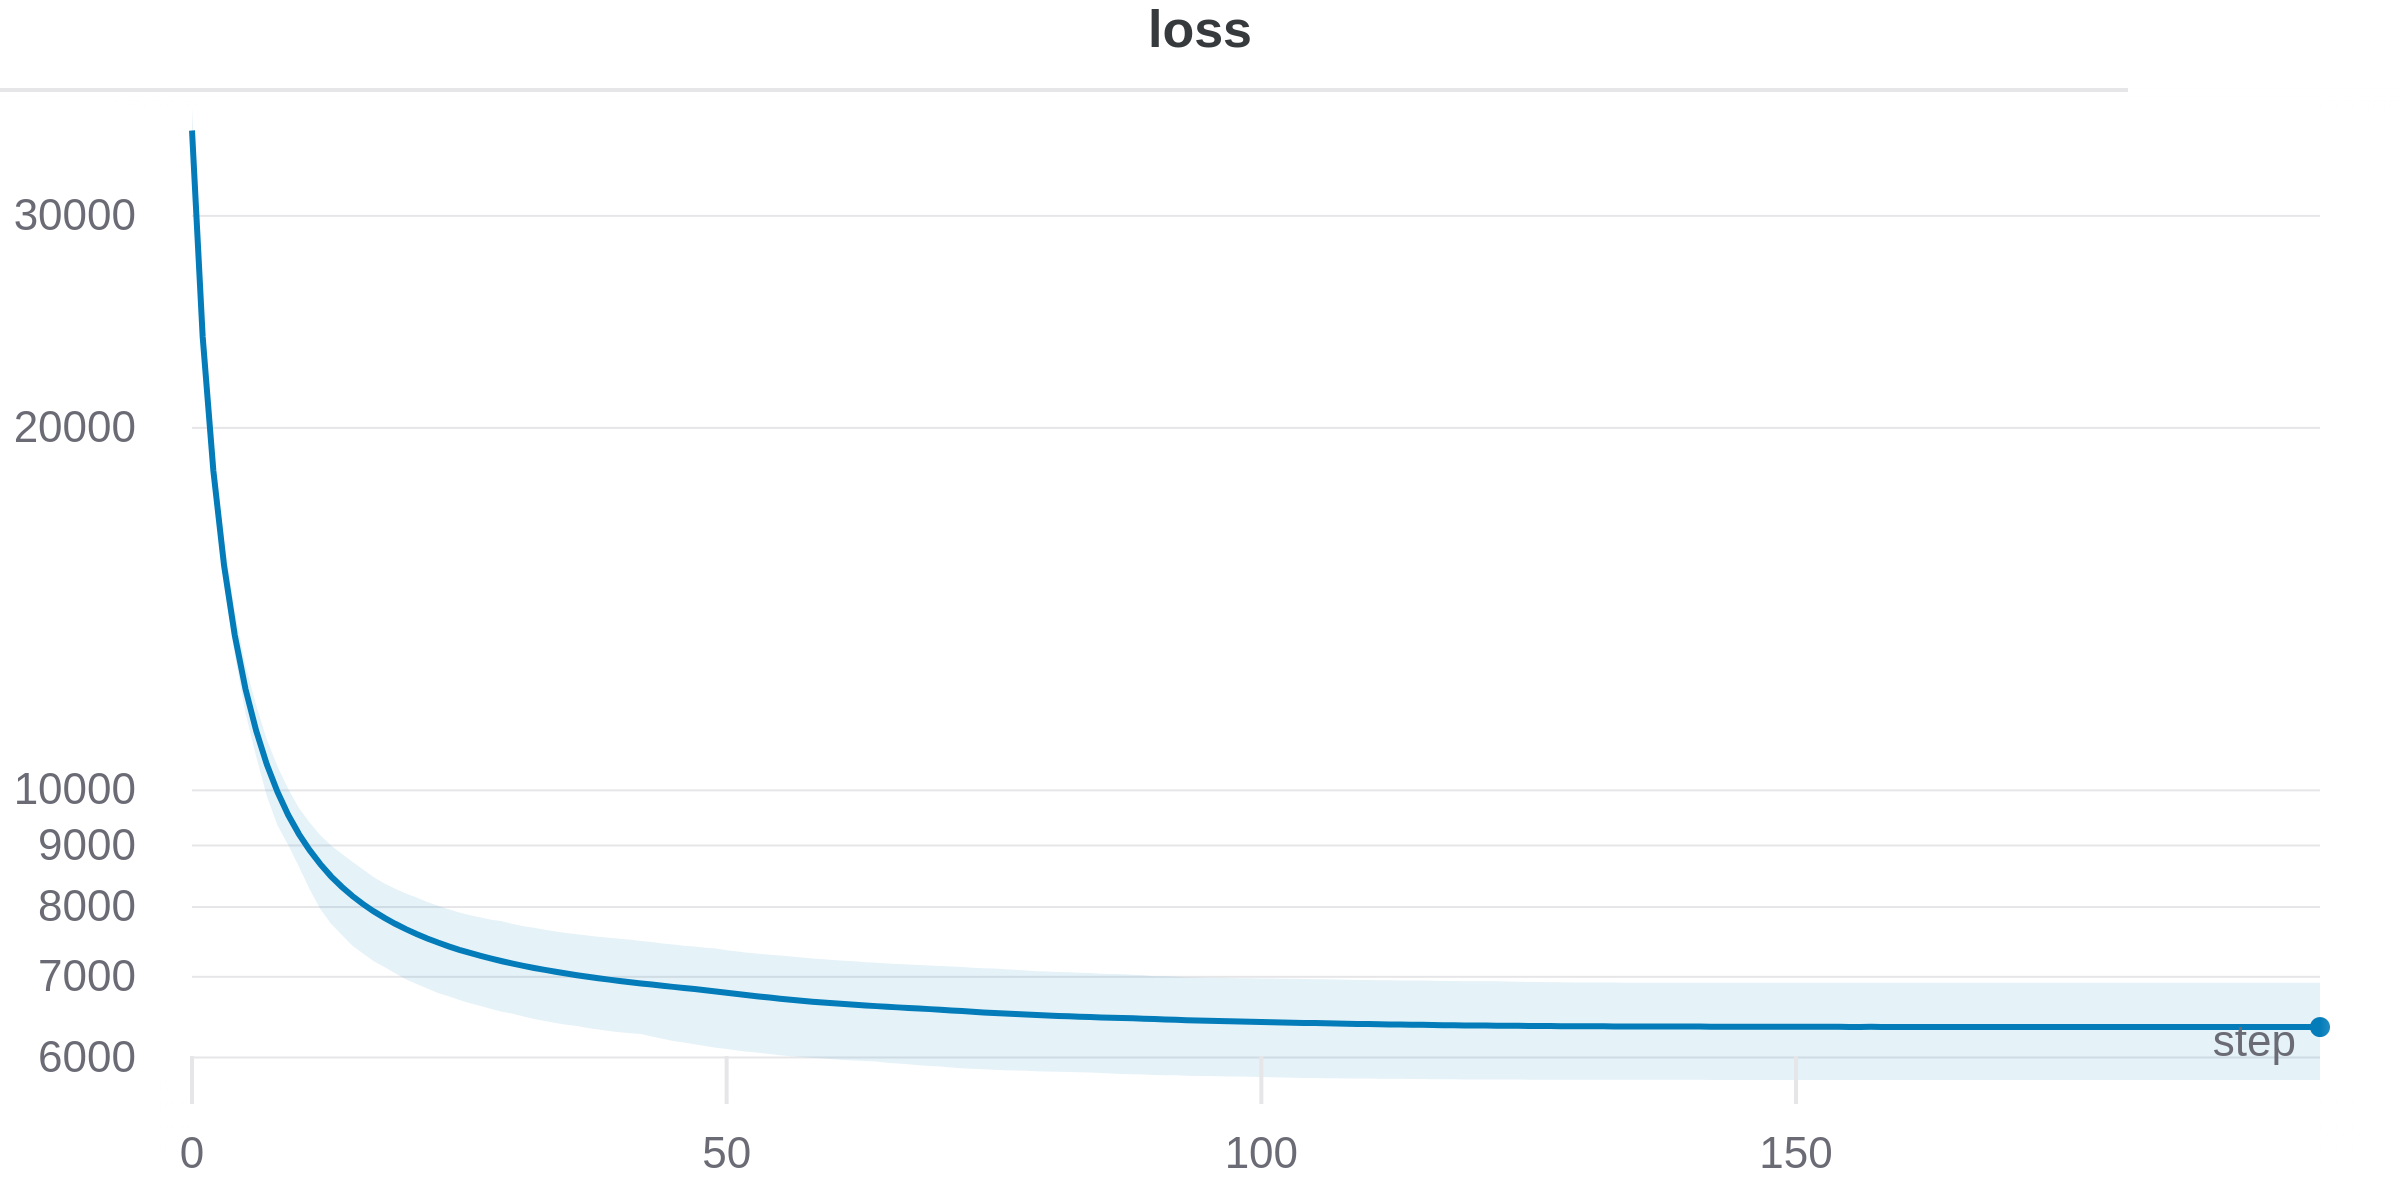
\includegraphics[width=0.8\textwidth]{images/optimization_curve.png}
    \caption{Optimization curve of Algo. \ref{algo:gpu_hill_climbing}. Averaged over 100 independent runs.}
    \label{fig:gpu_hill_climbing}
\end{figure}

GPU augmented hill climbing method is fast enough to get reasonable good results in less than one minute.
One of the results can be visualized in Fig. \ref{fig:optimization_results}.

\begin{figure}
    \centering
    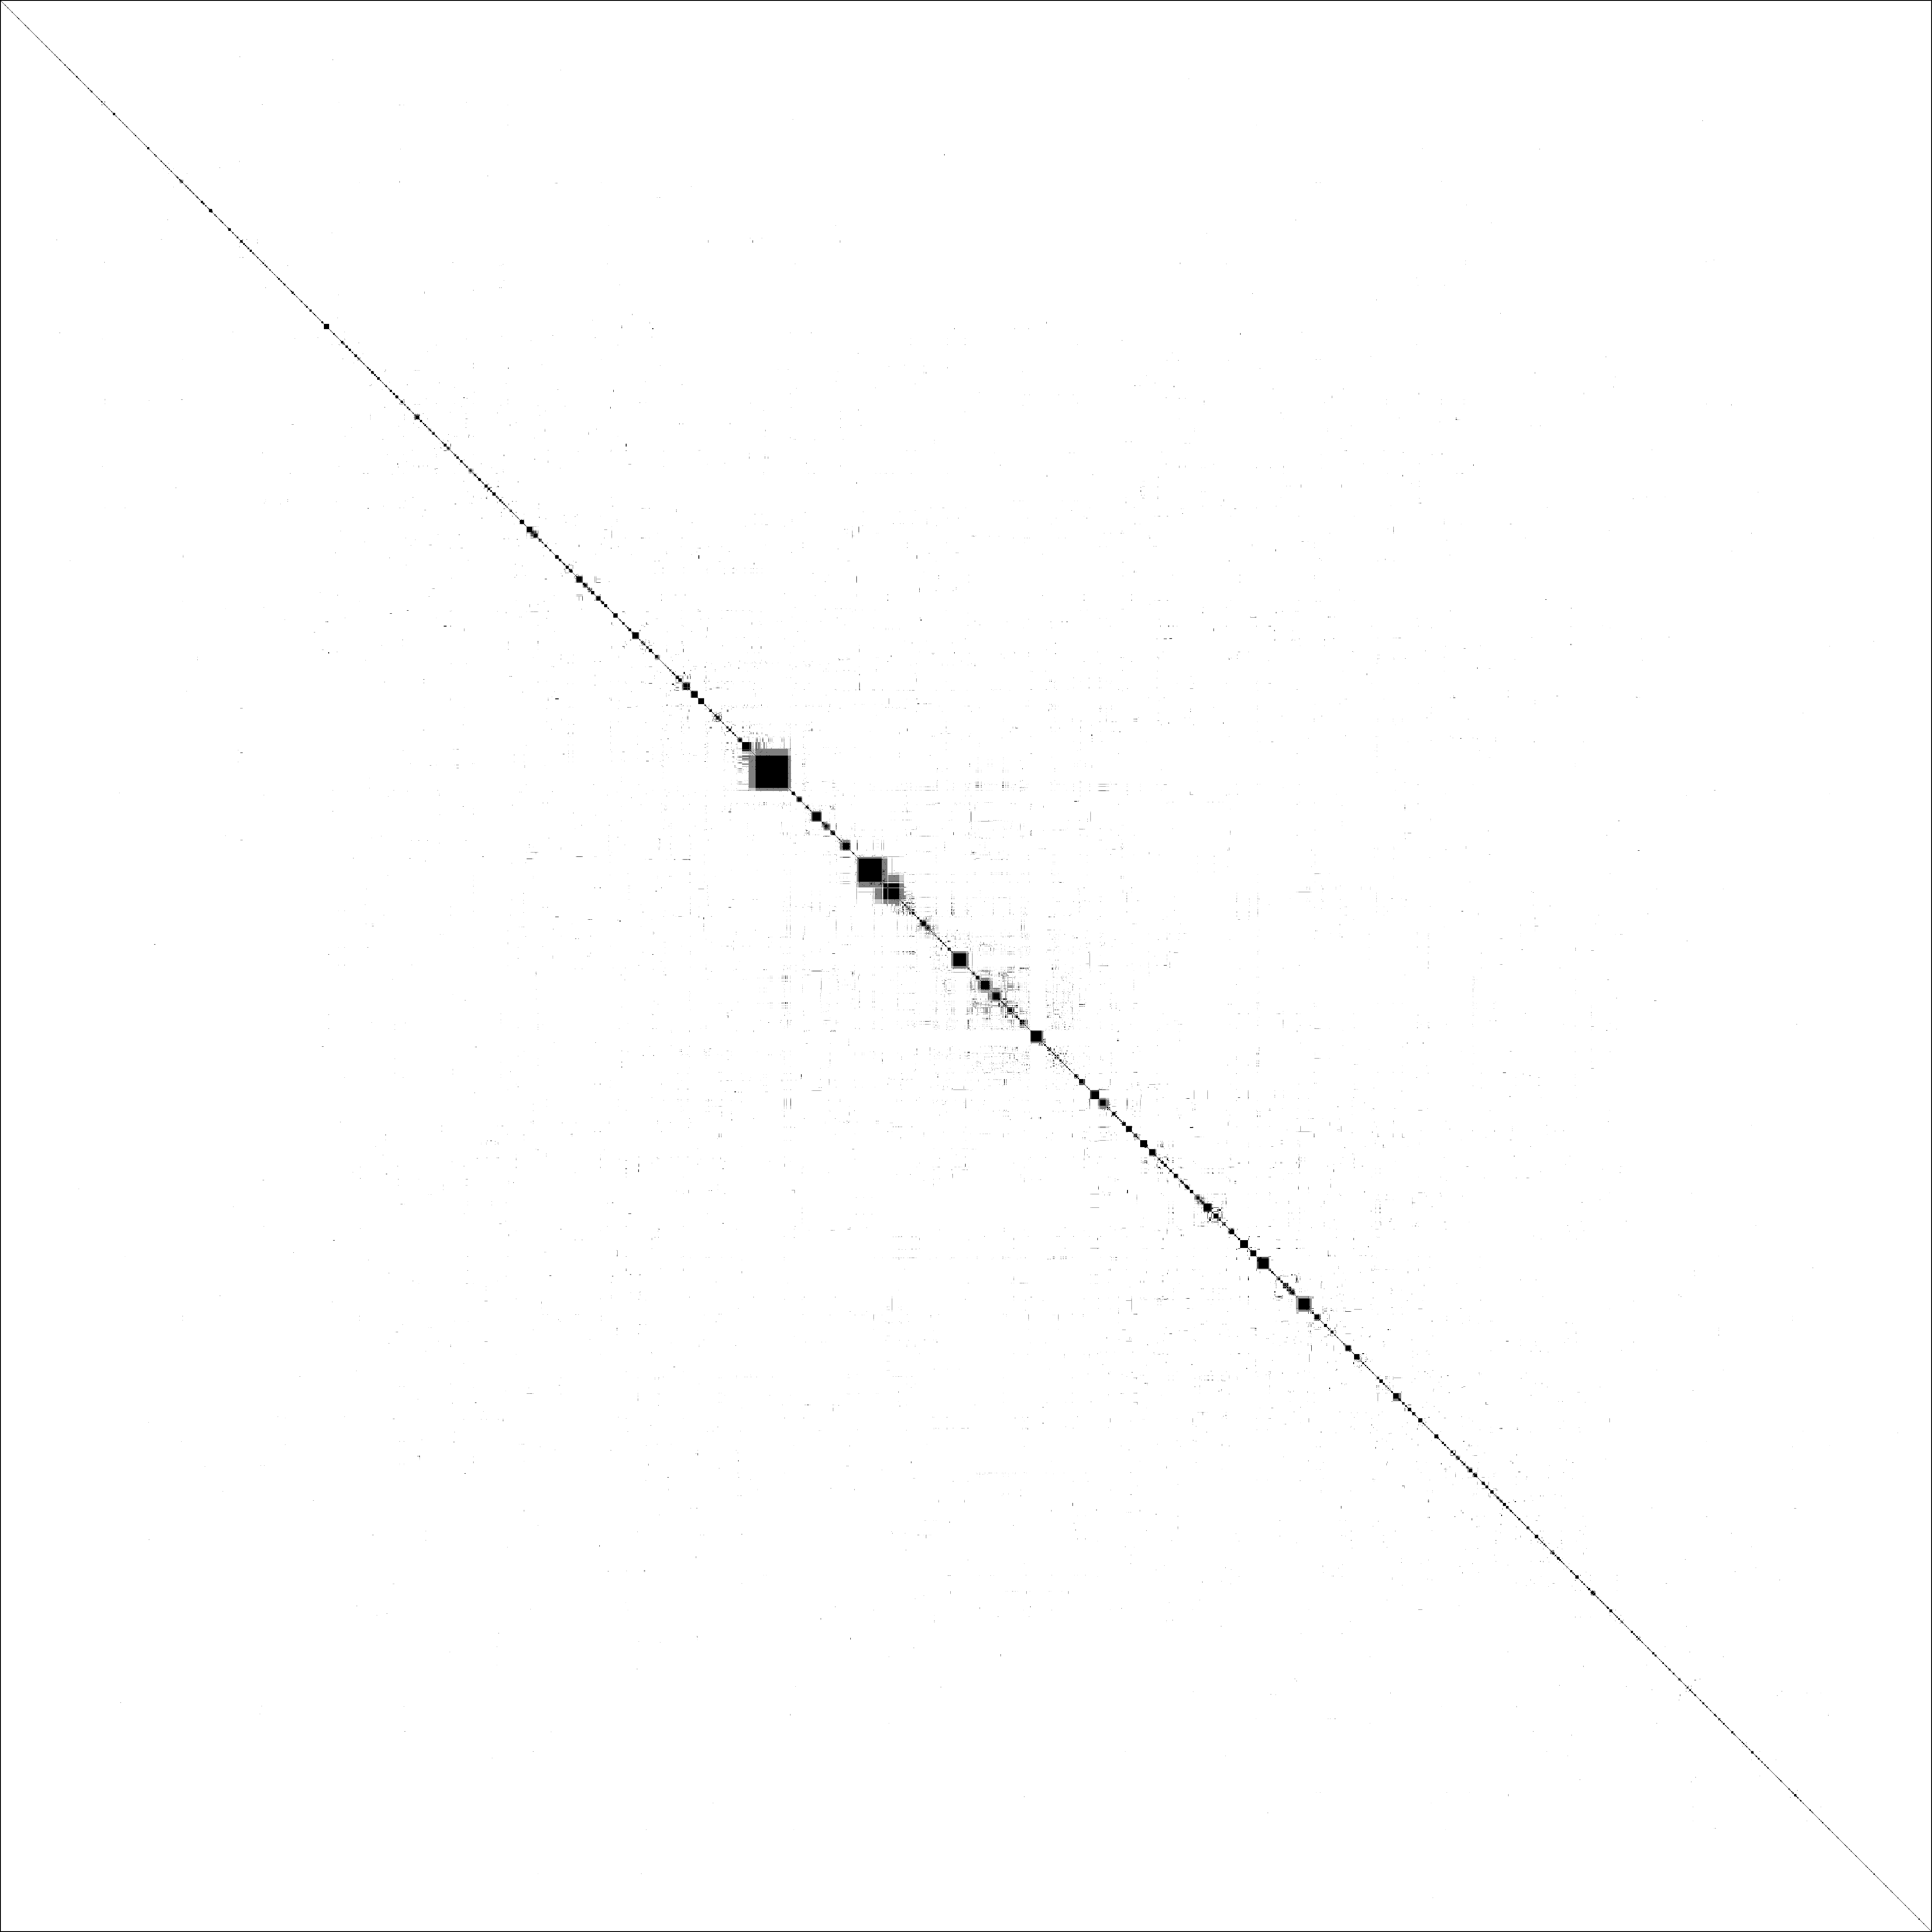
\includegraphics[width=\textwidth]{images/optimized_arrangement.png}
    \caption{The most optimal solution of Algo. \ref{algo:gpu_hill_climbing} in 100 runs.
    Comparing to the random arrangement in Fig. \ref{fig:matrix_random_arrangement}, 
    now we can easily observe the structure of the research community.
    }
    \label{fig:optimization_results}
\end{figure}

However, it still slightly suffers from local optima.
In order to get more optimal results, one can not rely on running the algorithm for longer.

Our best results are achieved by searching with 100 independent runs with random initialization.
However, we observe that the initial states matter more than trying different choices during optimization.
Thus, an evolutionary approach \cite{eppley2001} searching for better initial states might be better than our random initialization.
